\section{Fortune's algorithm}
In this section we will present an algorithm which computes $\Vor(P)$ in $\mathcal{O}(n \log n)$ time. First, we need some assumptions:

\begin{assume} \label{ass:generalposition}
The points in $P$ are in general position, which we define to mean that no two points in $P$ have the same $x$-coordinate or the same $y$-coordinate.
\end{assume}

\begin{rmk}
We may make the above assumption without loss of generality, because if $\Theta \subset \R$ is the set of all of the angles that $\overline{p_i p_j}$ make with the $x$-axis for all $p_i \ne p_j$ in $P$, then $\Theta$ is finite and $\R \setminus \Theta$ is infinite, so generating a random number $\theta \in \R \setminus \Theta$ and letting
\[
    \varphi (x, y) = \begin{pmatrix} \cos \theta & -\sin \theta \\ \sin \theta & \cos \theta \end{pmatrix} \begin{pmatrix} x \\ y \end{pmatrix}
    = (\cos(\theta) x - \sin(\theta) y, \sin(\theta) x + \cos(\theta) y)
\]
be the rotation about the origin with the angle $\theta$, then the set
\[
    \varphi(P) = \makeset{\varphi(p)}{p \in P}
\]
is in general position with probability 1. After having computed the Voronoi diagram for $\varphi(P)$, we may then rotate the diagram by the angle $-\theta$ to obtain $\Vor(P)$.
\end{rmk}

\begin{assume} \label{ass:notsameline}
The points in $P$ do not all lie on the same line.
\end{assume}

\begin{rmk}
If $P$ is collinear then every point $p \in P$ lies on a line $\ell$. Theorem \ref{prop:structureofentirevoronoidiagram} gives us that $\VorG(P)$ consists of parallel lines and Theorem \ref{thm:characterizationofbisectors} gives us that these parallel lines are the bisectors of pairs of adjacent points on $\ell$. By sorting the points on $P$ along $\ell$ and then marking all the bisectors between adjacent points we then compute the Voronoi diagram of $\VorG(P)$ in $\mathcal{O}(n \log n)$ time. With this out of the way, it is now reasonable to make the above assumption.
\end{rmk}

Before we begin, we show that:

\begin{thm} \label{thm:voronoicansort}
The optimal worst-case running time for computing $\Vor(P)$ is $\mathcal{O}(n \log n)$.
\end{thm}
\begin{proof}
Let $A = \curly{a_1, a_2, \ldots, a_n} \subset \R$ and assume that $n \geq 3$. Define $\varphi \colon \R \to \R^2$ given by $\varphi(x) = (x, x^2)$. Now assume we have used an algorithm to compute a Voronoi diagram of the points
\[
    P = \varphi(A) = \curly{(a_1, a_1^2), (a_2, a_2^2), \ldots, (a_n, a_n^2)}.
\]
We obtain a diagram which looks similar to this:
\[
    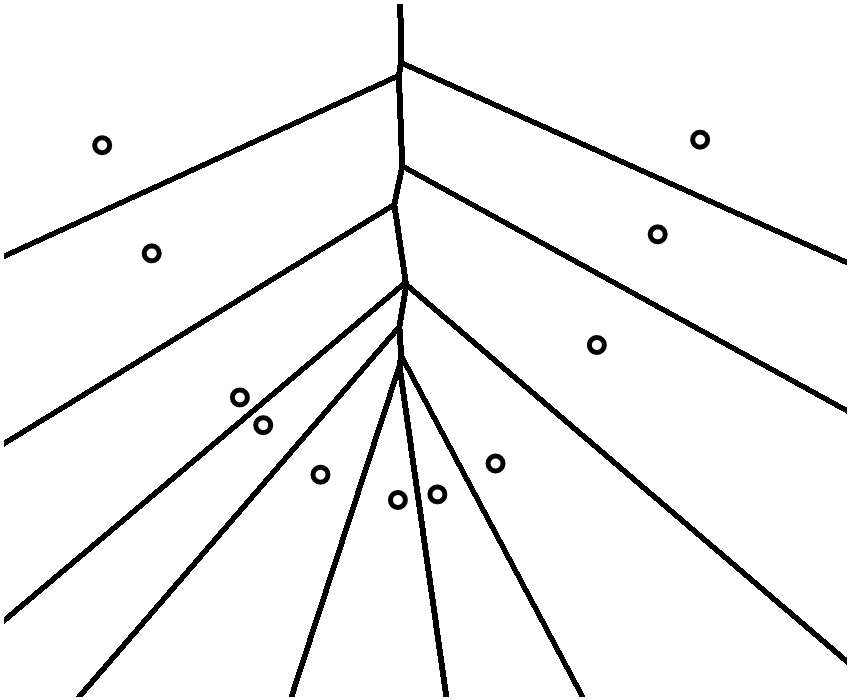
\includegraphics[scale=0.2]{voronoi-sorting-2}
\]
We may assume without loss of generality that $a_i \geq 0$ for all $i$, since we may just add
\[
    \max\makeset{-a}{a \in A \cup \curly{0} \text{ and } a \leq 0}
\]
to every number in $A$. Now we claim that
\begin{equation} \label{goodsortingproperty}
    0 \leq a < b < c < d < e
    \implies
    \begin{cases}
        \dist(\varphi(c), \varphi(b)) < \dist(\varphi(c), \varphi(a)) & \text{ } \\
        \quad\quad\quad\quad\quad\quad \text{ and } \quad & \text{ } \\
        \dist(\varphi(c), \varphi(d)) < \dist(\varphi(c), \varphi(e)). & \text{ }
    \end{cases}
\end{equation}
We have
\[
    \dist(\varphi(x), \varphi(y))^2 = \norm{\varphi(x) - \varphi(y)}^2 = (x - y)^2 + (x^2 - y^2)^2
\]
so
\[
    \dist(\varphi(c), \varphi(b)) < \dist(\varphi(c), \varphi(a))
\]
if and only if
\[
    \underbrace{(c - a)^2 - (c - b)^2}_{\lambda} + \underbrace{(c^2 - a^2)^2 - (c^2 - b^2)^2}_{\mu} > 0.
\]
The fact that $x \mapsto x^2$ is strictly increasing on $[0, \infty)$ and $0 \leq a < b < c$ implies that $\lambda > 0$ and $\mu > 0$. Using a similar argument, we obtain that $\dist(\varphi(c), \varphi(d)) < \dist(\varphi(c), \varphi(e))$. Thus (\ref{goodsortingproperty}) holds.

Now let $B = (b_1, b_2, \ldots, b_n)$ denote $A$ in sorted order, i.e. $i < j$ implies $b_i < b_j$. We'll now see how we can recover $B$ using $\Vor(P)$. We assume that the algorithm outputs a DCEL $\Delta$ of $\Vor(P)$. The property (\ref{goodsortingproperty}) implies that $\partial \mathcal{V}(\varphi(b_i))$ and $\partial \mathcal{V}(\varphi(b_j))$ share an edge when $i = j + 1$. This means that given $\mathcal{V}(\varphi(b_i))$ for $i < n$ we may find $b_{i+1}$ by traversing the edges of $\mathcal{V}(\varphi(b_i))$ in $\Delta$ until we find the face which belongs to $b_{i+1}$. We identify this face as the one which minimizes $a_j - b_i > 0$ where $\mathcal{V}(\varphi(a_j))$ is an adjacent face. In linear time we may find $\ell$ such that $a_{\ell} < a_i$ for all $i \ne \ell$. Let $b_1 := a_{\ell}$. Now assume that $b_i = a_j$ for $i < n$ and some $j$, and that we have the face $F = \mathcal{V}(\varphi(a_j)) \in \Delta$. We traverse the edges of $F$ until we find the face $F' = \mathcal{V}(\varphi(a_k)) \in \Delta$ which belongs to $b_{i+1}$, and we let $b_{i+1} := a_k$. In the worst case we iterate through every edge of every face of $\Delta$, but Remark \ref{rmk:boxalsohaslinearnumedges} gives us that there is $\mathcal{O}(n)$ edges in total, so we find all the $b_i$ in linear time. This means we can use an algorithm which computes $\Vor(P)$ to sort, which proves the claim.
\end{proof}
\todo{Choose a computation model in order for the above to make sense.}

Fortune's algorithm is a sweep line algorithm which maintains a horizontal sweep line $\ell \colon y = \ell_y$, and $\ell$ sweeps the plane from top to bottom in order to uncover the structure of the Voronoi diagram. 

For a point $p = (p_x, p_y) \in \R^2$ and a sweep line $\ell \colon y = \ell_y$ the distance between $p$ and $\ell$ is
\[
    \dist(p, \ell) = \abs{p_y - \ell_y}.
\]
Define
\[
    B_i = \makeset{q \in \R^2}{\dist(q, p_i) = \dist(q, \ell)}
\]
for all $i$. If $(p_i)_y > \ell_y$, it turns out we may parametrize $B_i$ by a parabola: Let $p = (p_x, p_y)$ denote $p_i$ and let $q = (x, y) \in B_i$. Since distances are non-negative, it is equivalent to looking at satisfying $\dist(q, p)^2 = \dist(q, \ell)^2$. We have:
\[
    \dist(q, p)^2 = \dist(q, \ell)^2 \iff (p_x - x)^2 + (p_y - y)^2 = (y - \ell_y)^2.
\]
This can be transformed into the equation
\begin{equation}
    2 (p_y - \ell_y) y = x^2 - 2 p_x x + p_x^2 + p_y^2 - \ell_y^2.
\end{equation}
Since $p_y \ne \ell_y$ by assumption, we obtain the parabola:
\begin{equation} \label{eq:parabola}
    y = \frac{1}{2 (p_y - \ell_y)} (x^2 - 2 p_x x + p_x^2 + p_y^2 - \ell_y^2),
\end{equation}
which parametrizes $B_i$ if $(p_i)_y > \ell_y$. Now we look at the situation where $(p_i)_y = \ell_y$. Then
\[
    \dist(q, p)^2 = \dist(q, \ell)^2 \iff (p_x - x)^2 + (p_y - y)^2 = (p_y - y)^2.
\]
Then it must be the case that $p_x = x$, so $B_i$ is a subset of a vertical line, and is a line segment if there is some $B_k$ above $B_i$ and a half-line which starts at $p_i$ otherwise. Finally, if $(p_i)_y < \ell_y$, we let $B_i = \varnothing$. We now for all $i$ define the maps
\[
    \beta_i(x) = \begin{cases}
        \displaystyle \frac{x^2 - 2 (p_i)_x x + (p_i)_x^2 + (p_i)_y^2 - \ell_y^2}{2 ((p_i)_y - \ell_y)} & \text{if } (p_i)_y > \ell_y, \\
        \infty & \text{otherwise.}
    \end{cases}
\]
Let $\textsf{LB}(x)$ denote the map which takes the minimum of each $\beta_i$, i.e.
\[
    \textsf{LB}(x) = \min\curly{\beta_1(x), \beta_2(x), \ldots, \beta_n(x)}.
\]
\begin{defn}[Beach line]
The \emph{beach line for the points $P$ with regards to the sweep line $\ell$} is given by the following subset of $\R^2$:
\[
    G \cup V,
    %\makeset{(x, \textsf{LB}(x)) \in \R^2}{\textsf{LB}(x) < \infty} \cup \makeset{B_i - \curly{(p_i)_x} \times (\textsf{LB}((p_i)_x), \infty)}{(p_i)_y = \ell_y}.
\]
where $G$ is the graph of $\textsf{LB}$ when it is finite
\[
    G = \makeset{(x, \textsf{LB}(x)) \in \R^2}{\textsf{LB}(x) < \infty},
\]
and $V$ is all the vertical parts not hidden behind other parabolas
\[
    V = \makeset{B_i - \curly{(p_i)_x} \times (\textsf{LB}((p_i)_x), \infty)}{i = 1, \ldots, n \text{ where } (p_i)_y = \ell_y}.
\]
\end{defn}
\begin{rmk}
From the definition we see that the beach line consists of parts of parabolas, and vertical line segments or half-lines. For this reason, it is easy to see that the intersection between any vertical line and the beach line has at most one component.
\end{rmk}
\begin{rmk}
For a sweep line $\ell$ which does not intersect any of the points in $P$, it follows from the definition of beach line that the map $\textsf{LB}(x)$ parametrizes the beach line. This was used to make a simple demo visualing the beach line, which can be found in $\boxed{\textsf{demos/beachline}}$.
\end{rmk}
\begin{defn}[Breakpoint]
Every point $q$ on the beach line such that $q \in B_i \cap B_j$ for two different $i, j$ is called a \textit{breakpoint}.
\end{defn}

\begin{figure}[H]
    \centering
    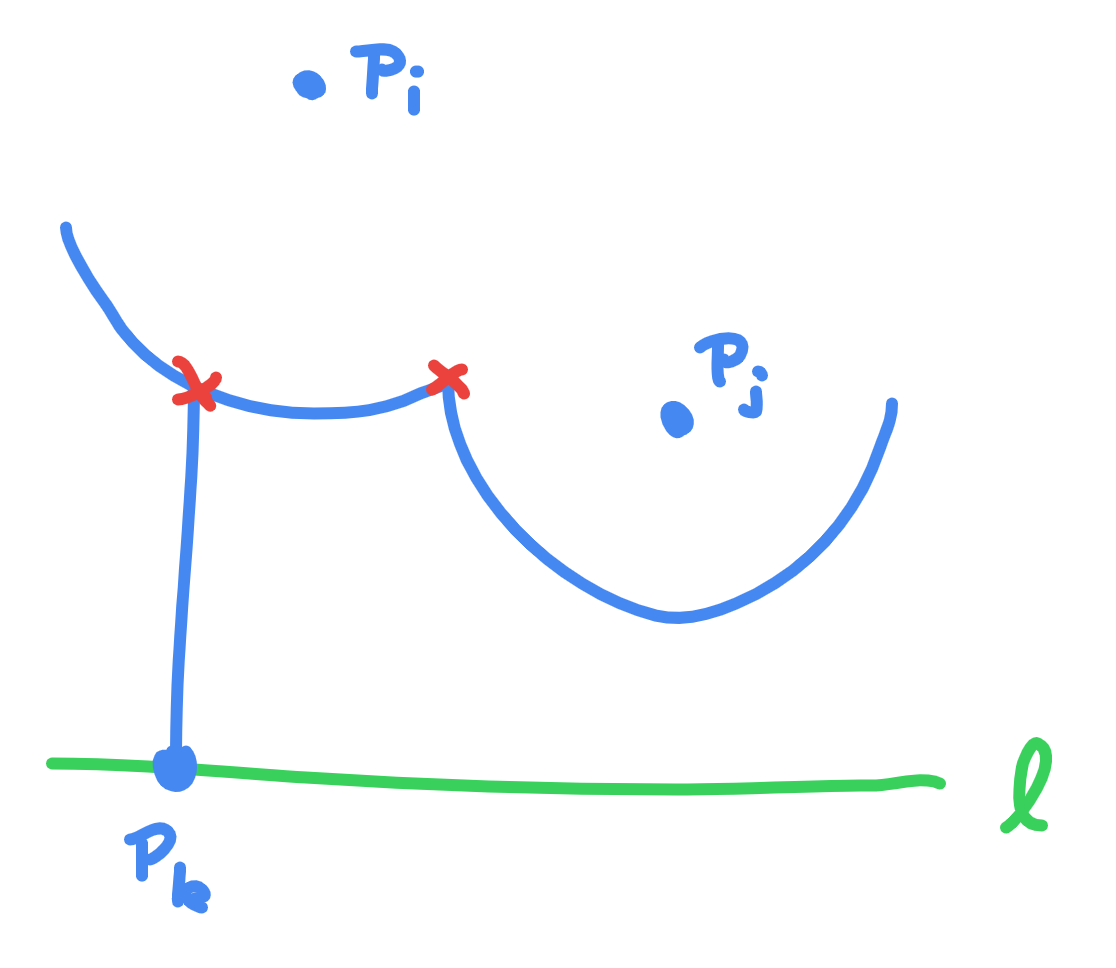
\includegraphics[scale=0.24]{temp-fig-6}
    \caption{The red crosses indicate breakpoints and the blue lines represent the beach line.}
    \label{fig:example-of-breakpoint}
\end{figure}

Now we show that the breakpoints exactly trace out $\VorG(P)$ as the sweep line $\ell$ moves from top to bottom.
\begin{prop}
We have the following:
\begin{enumerate}[{(}i{)}]
\item For every sweep line $\ell$: $y = \ell_y$ each breakpoint lies on $\VorG(P)$.
\item For every point $q$ in $\VorG(P)$ there is a position of the sweep line $\ell$ such that $q$ is a breakpoint.
\end{enumerate}
\end{prop}
\begin{proof}
We prove each statement individually:
\begin{enumerate}[{(}i{):}]
    \item Let $\ell$ be the sweep line, and assume that it has one or more breakpoints. Let $q \in \R^2$ be such a breakpoint. Then $q \in B_i \cap B_j$ for some $i \ne j$, which means that
    \[
        \dist(q, \ell) = \dist(q, p_i) = \dist(q, p_j).
    \]
    The last equality gives us that $q \not\in \mathcal{V}(p_k)$ for all $k$, hence $q \in \VorG(P)$.
    \item Let $q = (q_x, q_y) \in \VorG(P)$. Since $q$ is either an edge or a vertex, Theorem \ref{thm:characterizationofbisectors} gives us that $\partial C_P(q) \cap P$ has at least two elements, so let $p_i, p_j \in \partial C_P(q) \cap P$ be two different elements. We have $\dist(q, p_i) = \dist(q, p_j)$ by definition of $C_P(q)$, and then we may set
    \[
        \ell_y := q_y - \dist(q, p_i),
    \]
    and obtain
    \[
        \dist(q, \ell) = \dist(q, p_i) = \dist(q, p_j).
    \]
    Then $B_i$ and $B_j$ intersect at $q$, and $q$ is on the beach line since there is no $B_k$ with a point $p_k$ closer to $q$ than $p_i$ and $p_j$, by definition of $C_P(q)$.
\end{enumerate}
\end{proof}
As the sweep line $\ell$ sweeps the plane from top to bottom, the combinatorial structure of the beach line changes. We'll categorize these changes into \emph{events}.

First we will consider when new arcs appear on the beach line. As $\ell$ sweeps down and hits a point, a vertical segment is added to the beach line, and then as $\ell$ continues to move, the vertical line spreads out into a new parabolic arc, as seen in this figure:
\[
    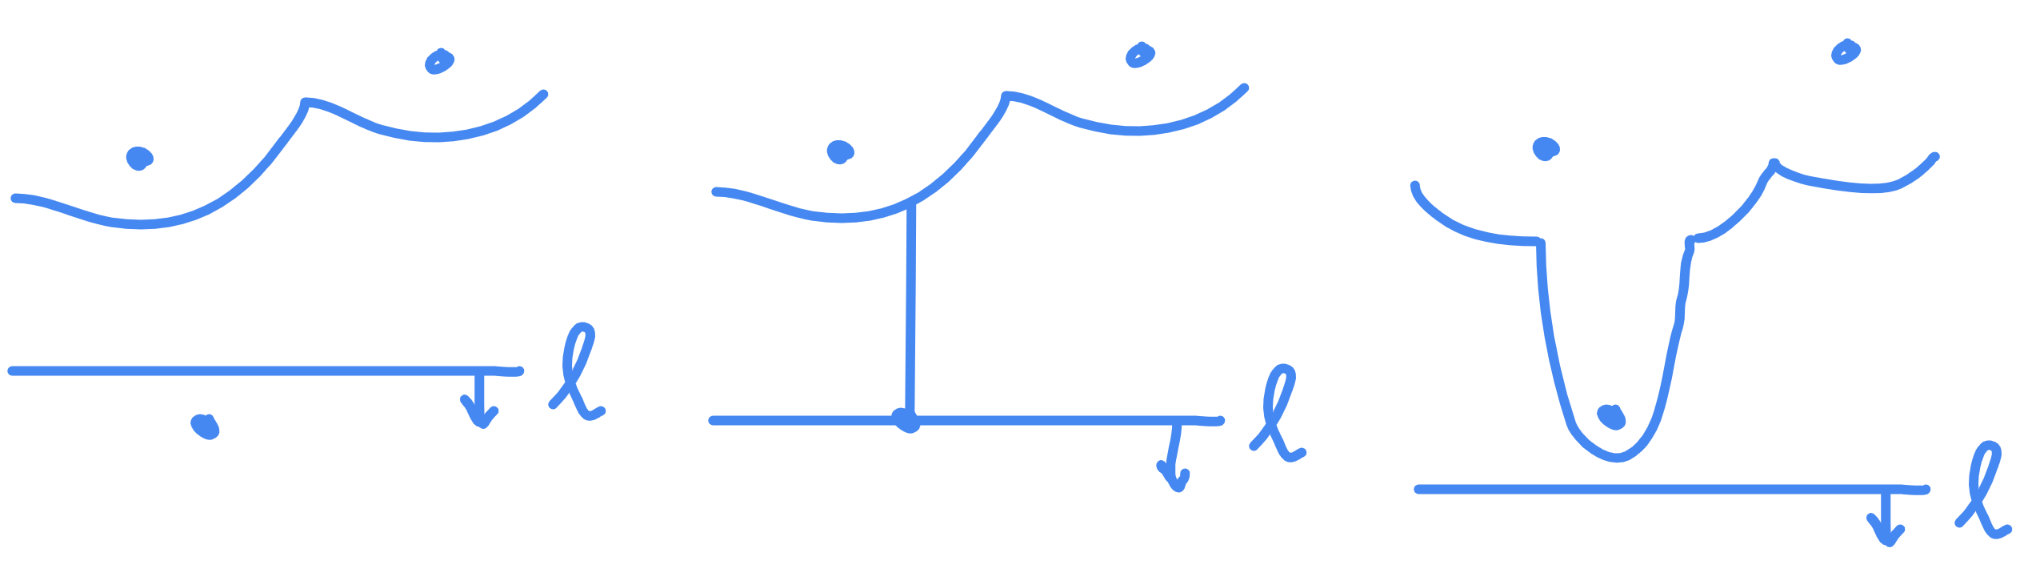
\includegraphics[scale=0.25]{temp-fig-7}
\]
\begin{defn}[Site event]
When $\ell$ encounters a point $p_i \in P$, that is when $\ell_y = (p_i)_y$, we say that we encounter a \emph{site event}.
\end{defn}
\begin{lem} \label{lem:newarciffsiteevent}
The only way in which a new arc can appear on the beach line is through a site event.
\end{lem}
\begin{proof}
The only other alternative is for new arcs to arise due to changes in the shape and position of existing parabolas, that is due to some parabola overtaking the beach line and breaking through it. Assume for the sake of a contradiction that a new arc appears on the beach line but $\ell_y \ne p_i$ for all $i$. Let $\beta_j$ denote the parabola which contains the new arc, associated to the point $p_j \in P$, which appears on the beach line. We have that $\beta_j$ is a full parabola since $\ell_y \ne p_j$. Now, we look at the two cases in which $\beta_j$ can appear as a new arc on the beach line.

The first possibility is that $\beta_j$ breaks through the middle of an another arc which is a part of the parabola $\beta_i$. For this to happen, there is a time at which $\beta_i$ and $\beta_j$ either coincide, or they are tangent which means they intersect in exactly one point which is on the beach line. They cannot coincide, since $p_i \ne p_j$, so they must intersect in exactly one point. By Assumption \ref{ass:generalposition} we have $(p_i)_y \ne (p_j)_y$ so $\beta_i(x) - \beta_j(x)$ is a second degree polynomial with discriminant
\begin{equation}
    D = \frac{(p_x - q_x)^2 + (p_y - q_y)^2}{(p_y - \ell_y)(q_y - \ell_y)}.
\end{equation}
Since $p_y, q_y > \ell_y$ the denominator is strictly positive, and since $p_i \ne p_j$ the numerator is also strictly positive, so $D > 0$. This means that $\beta_i$ and $\beta_j$ intersect in two different points, a contradiction.

The second possibility is that $\beta_j$ appears in between two arcs. Let these arcs be part of parabolas $\beta_i$ and $\beta_k$. Let $q$ be the intersection point between $\beta_i, \beta_j$ and $\beta_k$, and we assume that the arc on the beach line from $\beta_i$ is to the left of $q$, and the arc from $\beta_k$ is to the right of $q$, as in this figure:
\[
    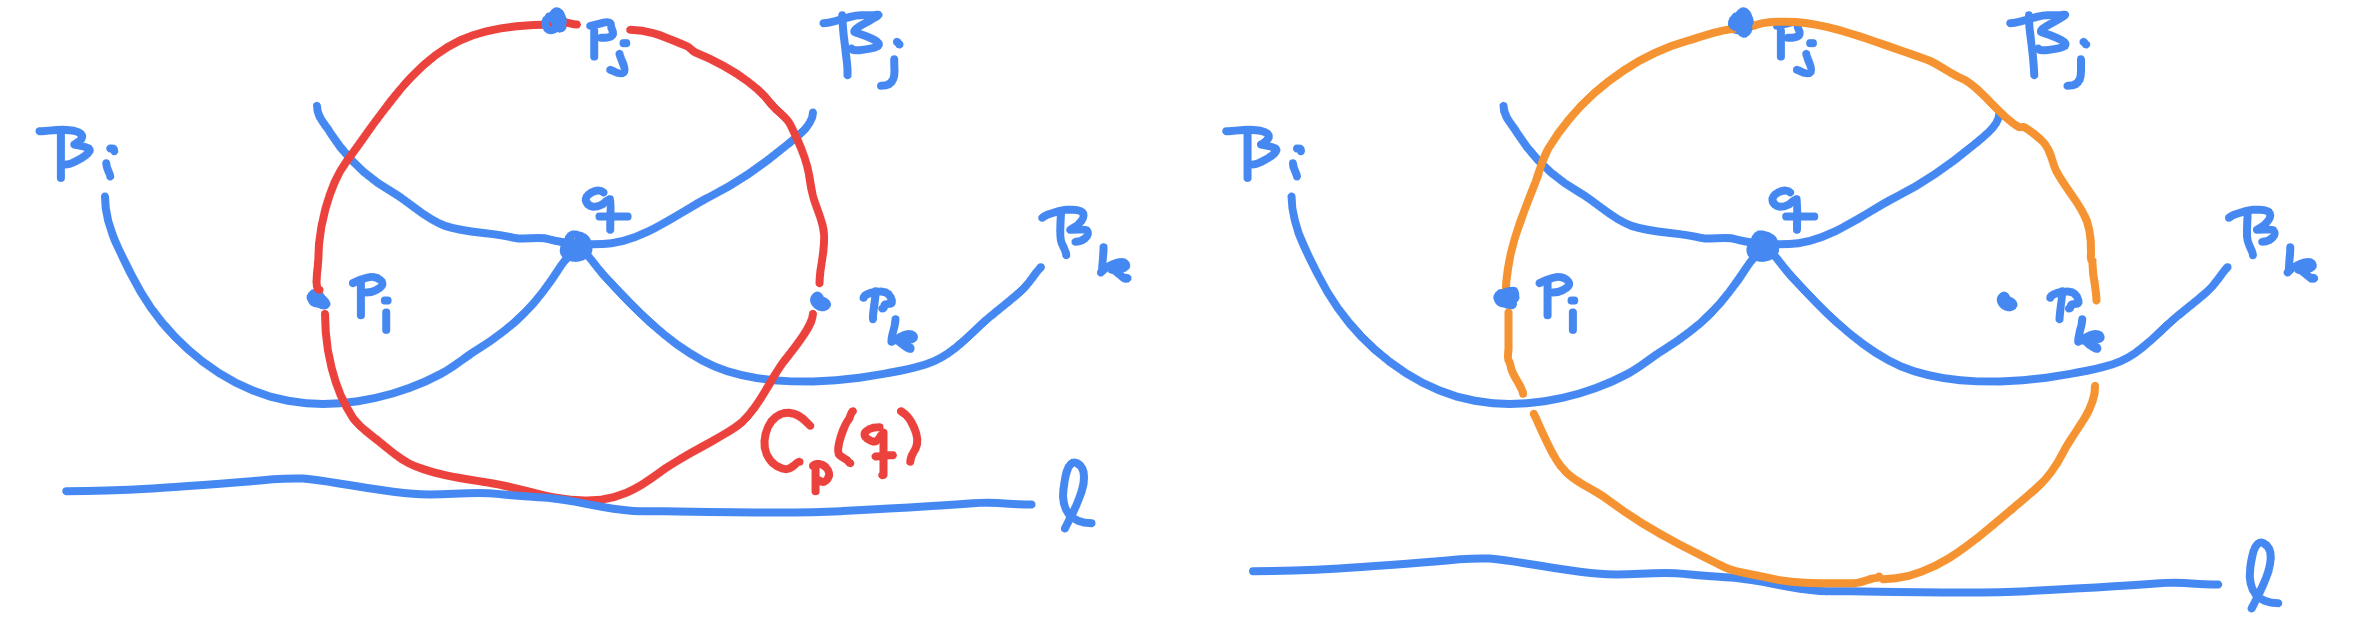
\includegraphics[scale=0.25]{temp-fig-8}
\]
Now let $C$ denote the circle $C_P(q)$ and note that it has $p_i, p_j, p_k$ on its boundary, and it is tangent to $\ell$. The cyclic order on $C$, starting at the point of tangency with $\ell$ and going clockwise is $p_i, p_j, p_k$. Now, we imagine an infinitesimal downward motion of $\ell$ while keeping $C$ tangent to $\ell$ and $p_j$, we call the new circle $C'$. Now either $p_i$ or $p_k$ will be contained in the interior of $C'$, say it's $p_k$ like on the figure. Let $c$ denote the center of $C'$. Then $\dist(c, p_j)$ is equal to $\dist(c, \ell)$, but since $p_k$ is contained in the interior of $C'$ then $\dist(c, p_k)$ is strictly smaller than $\dist(c, p_j)$, which means that $p_k$ is closer to $\ell$ than $p_j$, which means $\beta_j$ cannot be on the beach line, a contradiction.
\end{proof}

\begin{cor}
At any time the beach line consists of at most $2n-1$ arcs.
\end{cor}
\begin{proof}
We prove this by induction. The first site event adds a single arc, so for $n = 1$ there is at most $2n - 1 = 1$ arcs on the beach line. Now assume during the execution of the algorithm that we've seen $k < n$ of the $n$ site events, and that the beach line consists of at most $2k - 1$ arcs. When we encounter a new site, we have seen that there are two cases:
\[
    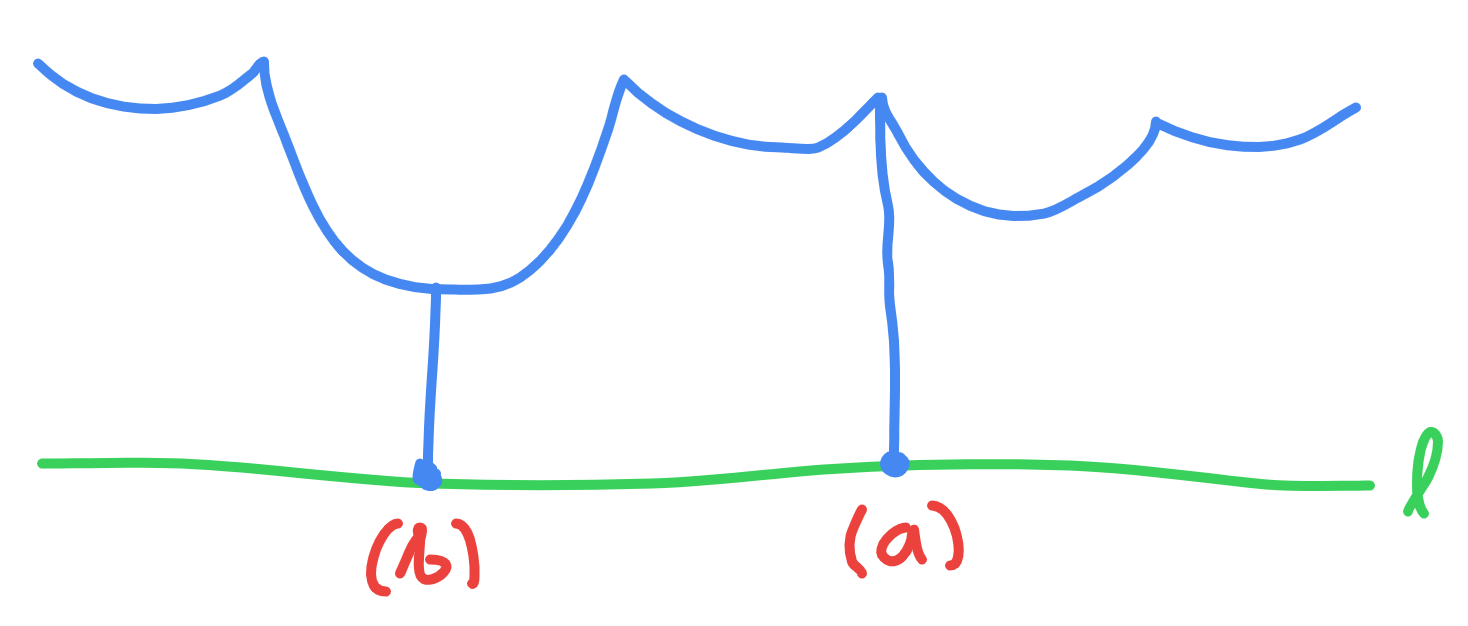
\includegraphics[scale=0.25]{temp-fig-11}
\]
In case (a) the have that an arc appears inbetween 2 existing arcs, increasing the total number by one. In case (b) an existing arc is split into two, and a new arc appears in between, which increases the total number by two. This means that after having seen $k + 1$ site events, there can be at most
\[
    (2k - 1) + 2 = 2(k + 1) - 1
\]
parabolic arcs, which proves the claim.
\end{proof}
Now we've characterized exactly when new arcs appear on the beach line. We now turn to the question of when arcs disappear from the beach line. Assume we have at least 3 arcs on the beach line, name them $\alpha, \alpha', \alpha''$ and assume that $\alpha$ is adjacent to $\alpha'$, and $\alpha'$ is adjacent to $\alpha''$. We assume that $\alpha'$ is the arc which is about to disappear. We first note that $\alpha$ and $\alpha''$ cannot be a part of the same parabola. If this case the case, we'd be in the following situation:
\[
    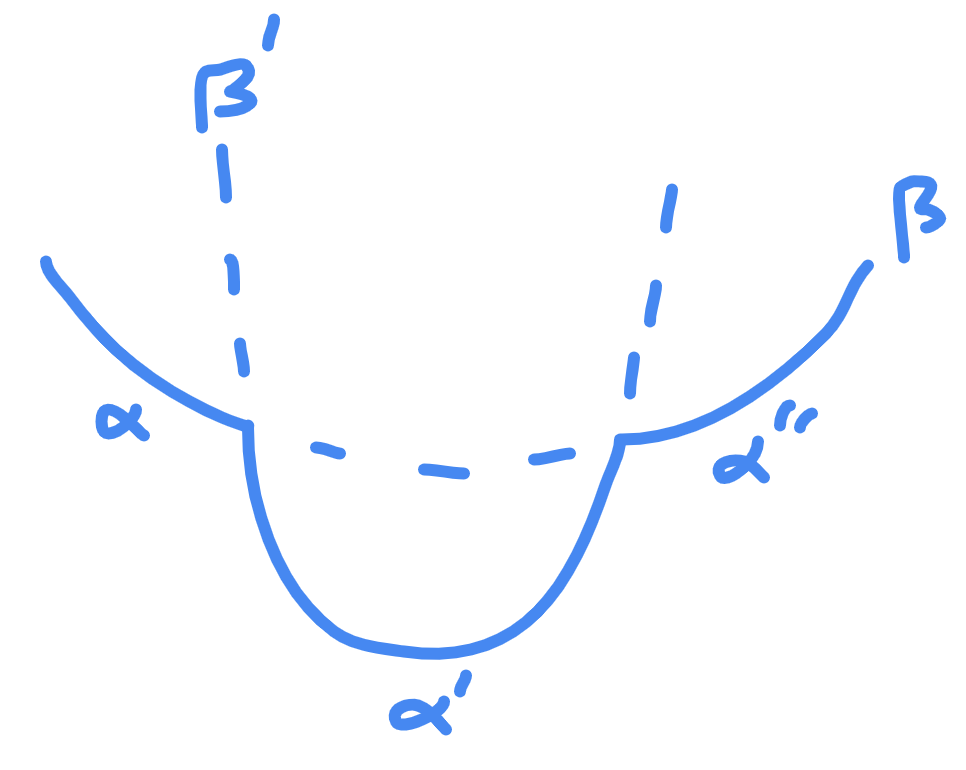
\includegraphics[scale=0.25]{temp-fig-12}
\]
Let $\beta$ denote the parabola which $\alpha$ and $\alpha''$ are a part of, and let $\beta'$ be the parabola which $\alpha'$ is a part of. When $\alpha'$ is about to disappear, then there will be a time at which $\beta$ and $\beta'$ are tangent, and then we can reuse the contradiction argument from the first part of the proof of Lemma \ref{lem:newarciffsiteevent}. Thus $\alpha, \alpha'$ and $\alpha''$ are defined by 3 distinct sites $p_i, p_j, p_k \in P$. At the moment that $\alpha'$ disappears, then the three parabolas $\beta_i \supset \alpha$, $\beta_j \supset \alpha'$ and $\beta_k \supset \alpha''$ intersect in a single point $q$. We note that
\[
    \dist(q, \ell) = \dist(q, p_i) = \dist(q, p_j) = \dist(q, p_k).
\]
So there is a circle $C$ with center $q$ passing through $p_i, p_j, p_k$ which is tangent to $\ell$ at its lowest point. The situation is illustrated as follows:
\[
    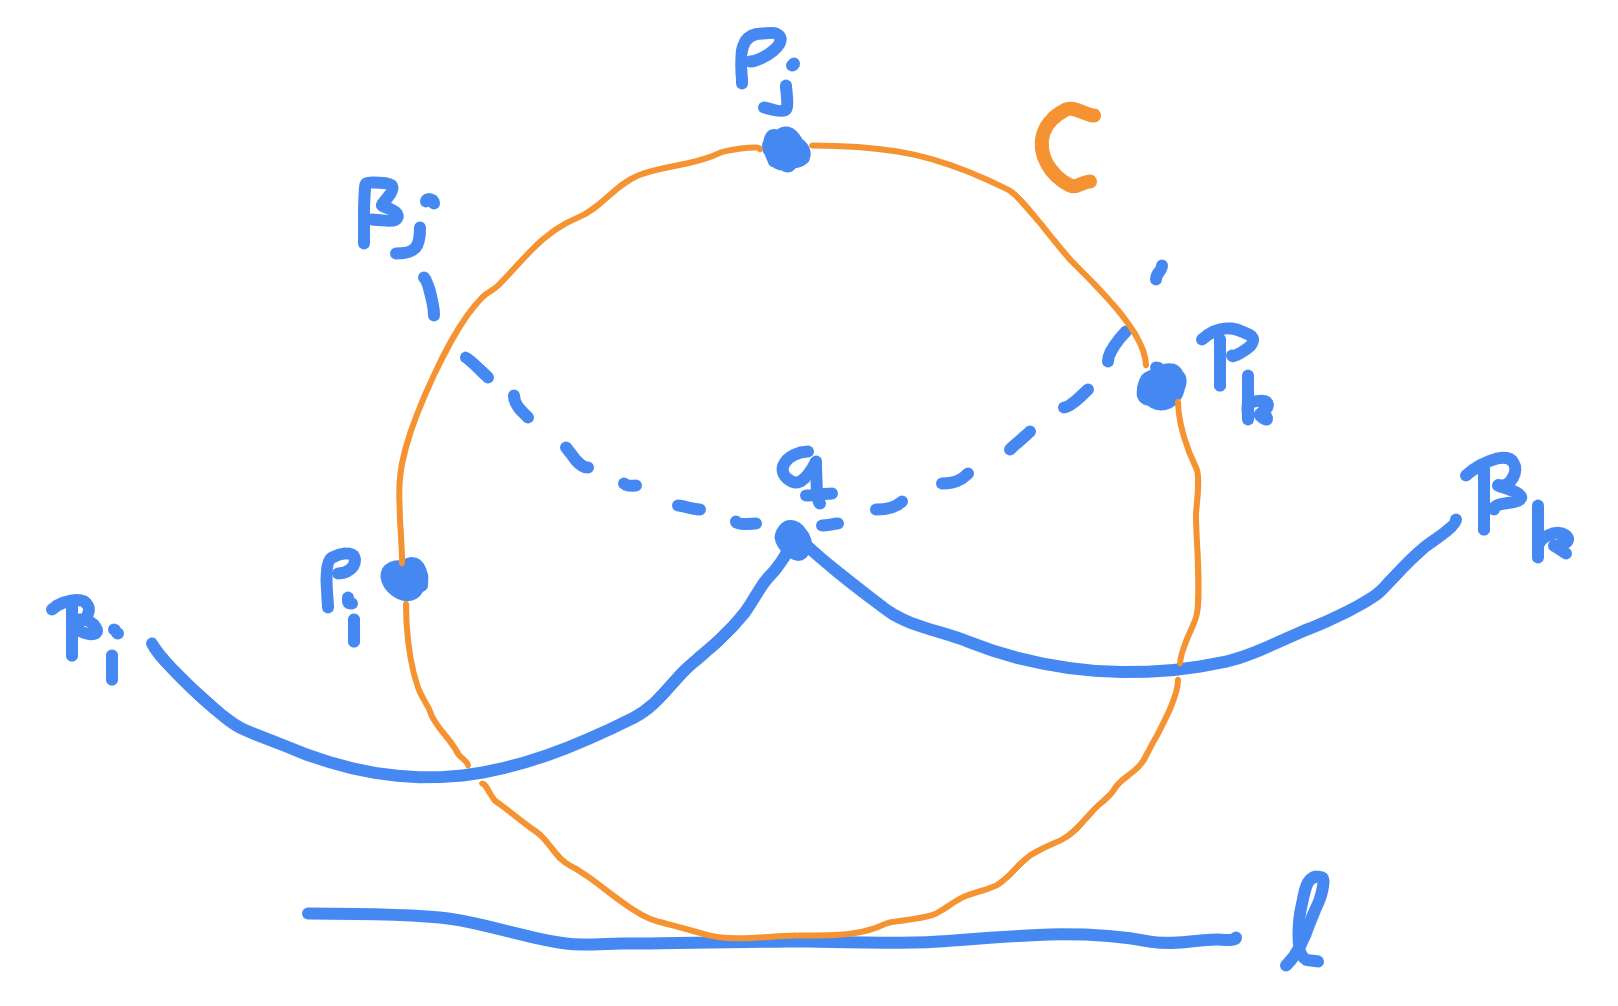
\includegraphics[scale=0.25]{temp-fig-13}
\]
We claim that $C = C_P(q)$. Assume for the sake of a contradiction that there is a site $p$ inside the interior of $C$. Then
\begin{equation} \label{eq:notonthebeachlinechar}
    \dist(p, q) < \dist(q, \ell).
\end{equation}
Now note the following characterization of being on the beach line: A point $r$ is on the beach line if $\dist(r, \ell) = \dist(r, p_i)$ for all $i \in \mathcal{I}$ and $\dist(r, \ell) < \dist(r, p_j)$ for all $j \in \mathcal{J}$, where $\mathcal{I}$ describes those indices $i$ where $r \in \beta_i$ and $\mathcal{J}$ describes those indices where $r \not\in \beta_j$. By assumption $q$ is on the beach line, since it is a point on all of $\alpha, \alpha', \alpha''$ but (\ref{eq:notonthebeachlinechar}) contradicts the characterization we just gave of the beach line. So it must be the case that $C = C_P(q)$. Now note that
\[
    \curly{p_i, p_j, p_k} \subset \partial C_P(q),
\]
so Theorem \ref{thm:characterizationofbisectors} (i) gives us that $q$ is a vertex of $\VorG(P)$. Compare this to the fact that breakpoints trace out $\VorG(P)$ as we proved earlier. This means that when two breakpoints meet and an arc disappears from the beach line, then two edges of $\Vor(P)$ meet at a vertex. We call the event when $\ell$ reaches the lowest point of a circle through three sites defining consecutive arcs on the beach line a \emph{circle event}. We have thus just proven:
\begin{lem}
The only way in which an existing arc can disappear from the beach line is through a circle event.
\end{lem}

\newpage
\begin{prop} \label{prop:highschool1}
Let $f(x) = a x^2 + b x + c$ be a polynomial with discriminant $D > 0$ with roots $r_1 < r_2$. Then $r = \tfrac{1}{2}(r_1 + r_2)$ is the only solution to $\displaystyle\frac{df}{dx}(r) = 0$ and the expressions $\displaystyle\frac{df}{dx}(r_1)$ and $\displaystyle\frac{df}{dx}(r_2)$ are non-zero and have opposite signs.
\end{prop}
\begin{proof}
It is well-known that we may factor $f$ as follows:
\[
    f = a (x - r_1) (x - r_2) = a x^2 - a(r_1 + r_2) x + a r_1 r_2.
\]
Since two polynomials are equal if and only if their coefficients are equal we get $b = - a (r_1 + r_2)$, which gives us
\[
    \frac{df}{dx} (r) = 2 a r + b = 2 a \para{\frac{r_1 + r_2}{2}} - a (r_1 + r_2) = 0.
\]
This is the only solution since $\displaystyle\frac{df}{dx}$ is a first degree polynomial. Now note that $\displaystyle\frac{d^2 f}{d x^2}(x) = 2a \ne 0$ and $r_1 < r < r_2$ which gives us that
\[
    \text{sgn} \para{\frac{df}{dx}(r_1)} = -\text{sgn} \para{\frac{df}{dx}(r_2)} \ne 0.
\]
\end{proof}
\todo{Put a cute geometrical proof of Proposition \ref{prop:highschool1} in a margin figure: Draw a parabola which intersects the $x$-axis twice at $r_1 < r_2$, and note that since the polynomial is symmetrical about its vertex, the expression $r = (r_1 + r_2)/2$ is immediate.}

Proposition \ref{prop:highschool1} will be used when we want to find out which arc on the beach line lies above a new point discovered through a site event. When intersecting two of the paraboals of the beach line, we will find two intersection points, because of our assumptions. Proposition \ref{prop:highschool1} then gives us that at these intersection points $r_1, r_2$ we have that
\[
    \begin{cases}
        \displaystyle\frac{d(\beta_i - \beta_j)}{dx}(r_k) \ne 0 \text{ for } k = 1, 2 & \text{ }\vspace{0.25cm} \\ \text{sgn} \para{\displaystyle\frac{d(\beta_i - \beta_j)}{dx}(r_1)} = -\text{sgn} \para{\displaystyle\frac{d(\beta_i - \beta_j)}{dx}(r_2)} & \text{ }
    \end{cases}
\]
We then want to locate a specific breakpoint between two arcs, and the above will help us to do this.

To intersect two parabolas $\beta_i$ and $\beta_j$ we write
\[
    (\beta_i - \beta_j)(x) = a x^2 + b x + c,
\]
where (for $p = p_i$ and $q = p_j$)
\begin{align*}
    a &= \frac{1}{2} \para{\frac{1}{p_y - \ell_y} - \frac{1}{q_y - \ell_y}}, \\
    b &= \frac{q_x}{q_y - \ell_y} - \frac{p_x}{p_y - \ell_y}, \\
    c &= \frac{\ell_y^2 (p_y - q_y) + p_x^2 q_y + p_y^2 q_y - p_y (q_x^2 + q_y^2) + \ell_y (q_x^2 + q_y^2 - p_x^2 - p_y^2)}{2 (p_y - \ell_y) (q_y - \ell_y)}.
\end{align*}
The square root of the discriminant is then
\[
    d = \sqrt{b^2 - 4 ac} = \sqrt{\frac{(p_x - q_x)^2 + (p_y - q_y)^2}{(p_y - \ell_y)(q_y - \ell_y)}}.
\]
The $x$-valuees of the intersection points are then given by the well-known formulas
\[
    r_1 = \frac{-b - d}{2 a}, \quad
    r_2 = \frac{-b + d}{2 a},
\]
which gives us the intersection points $q_1 = (r_1, \beta_i(r_1))$ and $q_2 = (r_2, \beta_i(r_2))$. Now, we want to find the breakpoint which at which an arc of $\beta_i$ exits the beach line, and an arc of $\beta_j$ enters the beach line, Proposition \ref{prop:highschool1} gives us a way of picking which one of $q_1$ and $q_2$ is the breakpoint that we need. For $\beta_i$ to exit and $\beta_j$ to enter, we need to pick $k$ such that
\[
    \frac{d \beta_i}{dx}(r_k) > \frac{d \beta_j}{dx}(r_k).
\]
Proposition \ref{prop:highschool1} garantuees that either
\begin{align*}
    \frac{d \beta_i}{dx}(r_1) > \frac{d \beta_j}{dx}(r_1) &\text{ and } \frac{d \beta_i}{dx}(r_2) < \frac{d \beta_j}{dx}(r_2) \\
    &\text{or} \\
    \frac{d \beta_i}{dx}(r_1) < \frac{d \beta_j}{dx}(r_1) &\text{ and } \frac{d \beta_i}{dx}(r_2) > \frac{d \beta_j}{dx}(r_2),
\end{align*}
so it is possible to make the right choice.

%GeoGebra demo of two points and their beach line
%\[
%    \boxed{\text{\url{https://www.geogebra.org/calculator/zreutrt6}}}
%\]